\documentclass[letterpaper]{article}
%\usepackage[pass,showframe]{geometry}

\usepackage{ijcai17}
\usepackage{times}
\usepackage{graphicx}
\usepackage{cleveref}

\usepackage[ruled,vlined]{algorithm2e}
\usepackage{MnSymbol,wasysym}
\usepackage{latexsym}
\usepackage{algpseudocode}
\usepackage{amsmath}

\usepackage{tikz}

\usetikzlibrary{graphs}

\newcommand{\citet}[1]{\citeauthor{#1} \shortcite{#1}}
\newcommand{\citep}[1]{\cite{#1}}

\newcommand{\AlgVar}[1]{\mathit{#1}}

\newcommand{\McSplit}{\textproc{McSplit}}

\newcommand{\nmax}{n_{\max}}

\newcommand{\lineref}[1]{line~\ref{#1}}
\newcommand{\linerangeref}[2]{lines~\ref{#1} to~\ref{#2}}
\newcommand{\Lineref}[1]{Line~\ref{#1}}
\newcommand{\Linerangeref}[2]{Lines~\ref{#1} to~\ref{#2}}

% TODO: use operatorname for these
\DeclareMathOperator{\V}{V}
\DeclareMathOperator{\E}{E}
\DeclareMathOperator{\N}{N}
\DeclareMathOperator{\vtxlabel}{label}

\newcommand{\BigO}[1]{\ensuremath{\operatorname{O}\left(#1\right)}}

%\newcommand{\examplexG}[5] {
%    \begin{minipage}{.2\textwidth}
%    \tikz {
%        \graph [nodes={draw, circle, minimum width=.6cm}, circular placement, radius=1cm,
%                clockwise=5] {
%                    1[label=90:#1],2[label=0:#2],3[label=0:#3],4[label=180:#4],5[label=180:#5];
%            1--4; 1--5; 2--3; 2--5; 3--5;
%        };
%    }
%    \end{minipage}
%}
%\newcommand{\examplexH}[6] {
%    \begin{minipage}{.2\textwidth}
%    \tikz {
%        \graph [nodes={draw, circle, minimum width=.6cm}, circular placement, radius=1.1cm,
%                clockwise=6, phase=60] {
%                    a[label=0:#1],b[label=0:#2],c[label=0:#3],d[label=180:#4],e[label=180:#5],f[label=180:#6];
%            a--b; a--c; a--e; b--d; b--f; c--d; c--e; c--f; d--f; e--f;
%        };
%    }
%    \end{minipage}
%}

\title{A Partitioning Algorithm for Maximum Common (Connected) Subgraphs\thanks{This work
was supported by the Engineering and Physical Sciences Research Council [grant
numbers EP/K503058/1 and EP/M508056/1]}}
\author{Ciaran McCreesh \and Patrick Prosser \and James Trimble \\
University of Glasgow, Glasgow, Scotland \\
j.trimble.1@research.gla.ac.uk}

\begin{document}

\maketitle

\begin{abstract}
    Maximium Common Subgraph (MCS) is the problem of finding a
    graph of maximium size that is an induced subgraph of each of the two input
    graphs.  We introduce \McSplit, a branch and bound algorithm that
    uses a vertex-labelling scheme to compactly represent the subsets of
    vertices that may be matched together to create a larger common subgraph.
    The new algorithm explores the same search space as the existing CP-FC
    algorithm, but requires only \BigO{n^2} space in total and \BigO{n} time
    for each recursive call, greatly improving on all existing algorithms for
    the problem.

    Experimental results using two large graph databases show that \McSplit\ is
    more than an order of magnitude faster than the leading existing algorithms
    on undirected, unlabelled graphs, including the problem
    variant in which the subgraph must be connected.
\end{abstract}

\section{Introduction}

Given graphs $G$ and $H$, the \emph{Maximum Common Subgraph (MCS)} problem is
to find a graph with as many vertices as possible that is isomorphic to induced
subgraphs of both $G$ and $H$. 

MCS has numerous applications, including finding the similarity between organic
molecules, \dots

This paper introduces a new branch and bound algorithm for MCS that improves
state-of-the-art run times on unlabelled, undirected instances by well over an
order of magnitude, and uses only quadratic memory in the order of the input
graphs, allowing us to solve larger instances than previously possible.

\section{Preliminaries}

We initially assume that $G$ and $H$ are unlabelled, undirected graphs without loops
(Section~\ref{sec:extensions} describes how these restrictions may be relaxed).

The vertices and edge sets of a graph $G$ are denoted $\V(G)$ and $\E(G)$.
The set of vertices adjacent to vertex $v$ in graph $G$ is called the
\emph{neighbourhood} of $v$, and denoted $\N(v, G)$.

We use $n_G$ and $n_H$ to denote $|\V(G)|$ and $|\V(H)|$. We will occasionally use
$n$ in complexity results to denote $n_G + n_H$.

\section{Prior Work}

The most successful existing approaches to solving MCS are reformulation to the
maximum clique problem on one hand \cite{DBLP:conf/cp/McCreeshNPS16}, and
constraint programming on the other \cite{DBLP:conf/cp/NdiayeS11}. In the
clique encoding, an association graph is created with one node for each pair in
the set $\{(u,v) \mid u \in \V(G), v \in \V(H) \}$ and an edge for each pair of
mappings that may be chosen together. A maximum clique in this graph
corresponds directly to a maximum common subgraph of $G$ and $H$.

In the constraint programming approach, we have a variable corresponding to
each vertex in $G$, and each variable initially has one value in its domain for
each vertex in $H$ to which it may be mapped, plus an additional value $\bot$
signifying that the vertex remains unmapped. A backtracking search is performed
in which values are assigned to variables, and propagation rules are used to
remove infeasible values from domains.  A matching algorithm is used to propagate
a soft $\mathit{allDifferent}$ constraint. ? Say this better

\section{The \McSplit\ algorithm}

This paper's main contribution is a branch and bound algorithm, \McSplit,
which uses a new vertex-labelling scheme to avoid explicitly maintaining the
set of feasible mappings for each vertex in $\V(G)$. As we will explore in
Section~\ref{sec:comparison}, the algorithm may be viewed as a version of the
constraint programming forward-checking (CP-FC) algorithm using a compact data
structure that exploits the nature of the MCS problem.  It is sufficiently
different, however, that it is helpful to describe the algorithm without
reference to previous approaches.

%At each node of the search tree, the algorithm
%labels vertices in $\V(G)$ and $\V(H)$ such that a pair $(v, w)$ with $v \in
%\V(G)$ and $w \in \V(H)$ can be added to the mapping if and only if $v$ and $w$
%have the same label.

The \McSplit\ algorithm finds a maximum-cardinality mapping $M^* = \{(v_1, w_1), \dots,
(v_{|M^*|}, w_{|M^*|})\}$, where the $v_i$ are distinct members of $\V(G)$ and the
$w_i$ are distinct members of $\V(H)$, such that $v_i$ and $v_j$ are adjacent
in $G$ if and only if $w_i$ and $w_j$ are adjacent in $H$. It is clear that,
given such a mapping, the subgraph of $G$ induced by $\{v_i, \dots, v_{|M^*|}\}$
and the subgraph of $H$ induced by $\{w_i, \dots, w_{|M^*|}\}$ are a maximum
common subgraph.

We will use the graphs $G$ and $H$ in Figure~\ref{fig:alg1} to demonstrate the
algorithm.  These graphs have a maximum common subgraph with four vertices; one
example is the mapping $\{1a, 2f, 3d, 5b\}$ (where vertex $1$ is assigned to
vertex $a$, $2$ is assigned to $f$, and so on).

\begin{figure}[ht]
\centering
    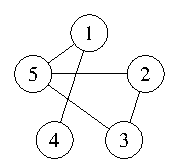
\includegraphics{graph_G}
    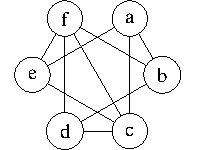
\includegraphics{graph_H}
%    \examplexG{}{}{}{}{}
%    \examplexH{}{}{}{}{}{}
\caption{Graphs $G$ and $H$}
\label{fig:alg1}
\end{figure}

The algorithm builds up a mapping $M$, starting with the empty mapping
$\emptyset$. Select a vertex in $\V(G)$ as the first vertex to be mapped; in
our example we will arbitrarily choose vertex $1$. Each of the vertices in
$\V(H)$ to which $1$ may be mapped will be tried in turn, and finally the
possibility where $1$ remains unmatched will be tried.

We will begin by mapping vertex $1$ to vertex $a$, giving $M=\{1a\}$.  Label
each unmatched vertex according to whether it is adjacent to $1$ (in $G$) or
$a$ (in $H$), as shown in Figure~\ref{fig:alg2}.  Adjacent vertices have label
1; non-adjacent vertices have label 0.  It is straightforward to see that we
can extend $M$ with a vertex mapping $vw$, with $v \in \V(G)$ and $w \in
\V(H)$, if and only if $v$ and $w$ have the same label.  This property that
two vertices may be mapped together if and only if they share a label is the
algorithm's main invariant.

\begin{figure}[ht]
\centering
\begin{minipage}[t]{0.15\linewidth}
    Mapping

    \bigskip

    $\{1a\}$
\end{minipage}
\quad
\begin{minipage}[t]{0.3\linewidth}
    Labelling of $G$
    \begin{tabular}[t]{cc}
    \hline
        Vertex & Label\\
    \hline
        $2$ & 0 \\
        $3$ & 0 \\
        $4$ & 1 \\
        $5$ & 1 \\
    \hline
    \end{tabular}
\end{minipage}
\quad
\begin{minipage}[t]{0.3\linewidth}
    Labelling of $H$
    \begin{tabular}[t]{cc}
    \hline
        Vertex & Label\\
    \hline
        $b$ & 1 \\
        $c$ & 1 \\
        $d$ & 0 \\
        $e$ & 1 \\
        $f$ & 0 \\
    \hline
    \end{tabular}
\end{minipage}
    \caption{Labels on vertices after mapping $1$ to $a$}
\label{fig:alg2}
\end{figure}

Next, extend the mapping by pairing a vertex in $G$ with a vertex in $H$ of the
same label; we will choose to map vertex $2$ to vertex $d$, giving $M=\{1a,
2d\}$ (Figure~\ref{fig:alg3}).  Each unmapped vertex $v \in \V(G)$ is labelled
with a two-character bit string, indicating whether $v$ is adjacent to each of
the two mapped vertices in $\V(G)$ (vertices $1$ and $2$).  For example, vertex
$3$ is labelled $01$, indicating that it is not adjacent to $1$ but is adjacent
to $2$.  Labels are given to unmapped vertices in $\V(H)$ in a similar fashion,
showing whether each vertex is adjacent to $a$ and $d$.

Our invariant is maintained: we can extend $M$ by a vertex pairing if
and only if the two vertices have the same label. Note also that each label is prefixed
by the label at the previous level of the search tree (Figure~\ref{fig:alg2}).

\begin{figure}[ht]
\centering
\begin{minipage}[t]{0.15\linewidth}
    Mapping

    \bigskip

    $\{1a, 2d\}$
\end{minipage}
\quad
\begin{minipage}[t]{0.3\linewidth}
    Labelling of $G$
    \begin{tabular}[t]{cc}
    \hline
        Vertex & Label\\
    \hline
        $3$ & 01 \\
        $4$ & 10 \\
        $5$ & 11 \\
    \hline
    \end{tabular}
\end{minipage}
\quad
\begin{minipage}[t]{0.3\linewidth}
    Labelling of $H$
    \begin{tabular}[t]{cc}
    \hline
        Vertex & Label\\
    \hline
        $b$ & 11 \\
        $c$ & 11 \\
        $e$ & 10 \\
        $f$ & 01 \\
    \hline
    \end{tabular}
\end{minipage}
\caption{After mapping $2$ to $d$}
\label{fig:alg3}
\end{figure}

The algorithm backtracks when the incumbent best mapping is at least as large
as a calculated bound given $M$ and the current labelling. To demonstrate how
this bound is calculated, we consider the situation one level deeper in the
search tree shown in Figure~\ref{fig:alg4}.

\begin{figure}[ht]
\centering
\begin{minipage}[t]{0.2\linewidth}
    Mapping

    \bigskip

    $\{1a, 2d, 3f\}$
\end{minipage}
\quad
\begin{minipage}[t]{0.3\linewidth}
    Labelling of $G$
    \begin{tabular}[t]{cc}
    \hline
        Vertex & Label\\
    \hline
        $4$ & 100 \\
        $5$ & 111 \\
    \hline
    \end{tabular}
\end{minipage}
\quad
\begin{minipage}[t]{0.3\linewidth}
    Labelling of $H$
    \begin{tabular}[t]{cc}
    \hline
        Vertex & Label\\
    \hline
        $b$ & 111 \\
        $c$ & 111 \\
        $e$ & 101 \\
    \hline
    \end{tabular}
\end{minipage}
\caption{After mapping $3$ to $f$}
\label{fig:alg4}
\end{figure}

Three vertex labels are used: 100,
101, and 111.  The first two of these only appear in one graph, and therefore
there is no way to add a pair of vertices with label 100 or 101 to the mapping.
The final label, 111, appears once in $G$ and twice in $H$, and therefore at
most one pair with this label can be added to $M$.  Thus, the upper bound on
matching size is $|M| + 1 = 4$. The general formula for the upper bound is
as follows, where $L$ is the set of labels used in both graphs.

\begin{multline*}
    \mathit{bound} = |M| + \sum_{l \in L} \min\big(|\{ v \in \V(G) : \vtxlabel(v)=l\}|, \\
        |\{ v \in \V(H) : \vtxlabel(v)=l \}|\big)
\end{multline*}


%When we have explored the full
%search space of matchings containing $\{1a, 2d\}$, we try reassigning $2$ to
%$f$.  Since $d$ and $f$ are the only vertices to which $2$ can be matched given
%the decision to match $1$ to $a$, we lastly explore the possibility that $2$ is
%left unmatched, by giving $2$ the label $\bot$ and selecting another vertex in
%$\V(G)$ to assign.

\paragraph{Efficient representation of label classes} The algorithm as
described so far requires $\BigO{n^2}$ space at each level of the search tree,
since labels may be up to $n_G$ bits in length. We can reduce the memory
requirement to $\BigO{n}$ per level by storing a pair $\langle P,T \rangle$ for
each label $l$ that is used, where $P$ is the set of vertices in $\V(G)$
labelled $l$, and $T$ is the set of vertices in $\V(H)$ labelled $l$. Since
there are $n_G + n_H$ vertices in the two graphs, at most $n_G + n_H$
label-classes can exist at once, and the total length of the $P$ and $T$ sets
is at most $n_G + n_H$.  We can gain further efficiency by discarding during
search any label-class that has an empty $P$ or $T$ set.

\begin{algorithm}
\DontPrintSemicolon
\nl $\FuncSty{expand}(\AlgVar{future},M)$ \;
\nl \Begin{
%\nl \lIf {$\AlgVar{future} = \emptyset$ \bf{and} $|M| > |\AlgVar{incumbent}|$}
\nl \lIf {$|M| > |\AlgVar{incumbent}|$}
    {$save(matching)$} \label{StoreIncumbent}
%\nl \lIf {$\AlgVar{future} = \emptyset$}{return}
\nl $bestFuture \gets 0$ \label{SetBestFutureToZero} \;
\nl \lFor {$\langle P,T \rangle \in \AlgVar{future}$}
    {$\AlgVar{bestFuture} \gets \AlgVar{bestFuture} + \min(|P|,|T|)$}
\nl \lIf {$|M|  + \AlgVar{bestFuture} \leq |\AlgVar{incumbent}|$}{return} \label{PruneSearch}
\bigskip
\nl $\langle P,T \rangle \gets \FuncSty{SelectLabelClass}(\AlgVar{future})$ \label{SelectClass} \;
\nl $v \gets \FuncSty{SelectVertex}(P)$ \label{SelectVertex} \;
\nl \For {$w \in T$ \label{WLoop}} {
\nl    $M \gets M \cup (v,w)$ \label{GrowM} \;
\nl    \bf{Let} $\AlgVar{future'} \gets \emptyset$ \label{NewFuture} \;
\nl    \For {$\langle P',T'\rangle \in future$ \label{InnerLoop}}{
\nl        \bf{Let} $P'' \gets P' \cap N(v,G) \setminus \{v\}$ \label{NewPWithEdge} \;
\nl        \bf{Let} $T'' \gets T' \cap N(w,H) \setminus \{w\}$ \;
\nl        \lIf {$P'' \neq \emptyset$ \bf{and} $T'' \neq \emptyset$}
        {$\AlgVar{future'} \gets \AlgVar{future'} + \langle P'' , T'' \rangle$ \label{AddToFutureWithEdge}}
\nl        \bf{Let} $P'' \gets P' \cap N(v,\overline{G}) \setminus \{v\}$ \label{NewPWithoutEdge}  \;
\nl        \bf{Let} $T'' \gets T' \cap N(w,\overline{H}) \setminus \{w\}$ \;
\nl        \lIf {$P'' \neq \emptyset$ \bf{and} $T'' \neq \emptyset$}
        {$\AlgVar{future'} \gets \AlgVar{future'} + \langle P'' , T'' \rangle$} \label{InnerLoopEnd}
       }
\nl   $\FuncSty{expand}(\AlgVar{future'},M)$ \label{ExpandWithV} \;
\nl   $M \gets M \setminus \{(v,w)\}$ \label{ShrinkM} \;
  }
\nl $P' \gets P \setminus \{v\}$ \label{RemoveV} \;
\nl $\AlgVar{future} \gets \AlgVar{future} \setminus \{\langle P,T \rangle\} \cup \{\langle P', T \rangle\}$\;
\nl \lIf {$P' = \emptyset$} {$\AlgVar{future} \gets \AlgVar{future} \setminus \{\langle P',T \rangle \}$}
\nl $\FuncSty{expand}(\AlgVar{future},M)$ \label{ExpandWithoutV} \;
}
\;
\nl $\FuncSty{McSplit}(G,H)$ \label{McSplitFun} \;
\nl \Begin{
\nl $\AlgVar{incumbent} \gets \emptyset$ \;
\nl $\FuncSty{expand}(\{\langle V(G),V(H) \rangle \},\emptyset)$ \label{FirstExpandCall} \;
\nl return $|\AlgVar{incubent}|$ \;
}
\caption{\McSplit\ algorithm for Maximum Common Subgraph}
\label{jtAlg}
\end{algorithm}

\paragraph{Full algorithm} The full algorithm is shown as
Algorithm~\ref{jtAlg}.  The recursive procedure, $\FuncSty{expand}$, has
two parameters.  The parameter $\AlgVar{future}$ is a list of label classes,
each represented as a $\langle P, T \rangle$ pair as described above.  The
parameter $M$ is the current mapping of vertices.  On each call to
$\FuncSty{expand}$, the invariant holds that a $(v,w)$ pair may be added to $M$
if and only if $v$ and $w$ belong to the same label class in $M$.

\Lineref{StoreIncumbent} stores the current mapping $M$ if it is large enough
to unseat the incumbent.  \Linerangeref{SetBestFutureToZero}{PruneSearch} prune
the search when a calculated upper bound ($\AlgVar{bestFuture}$) is not larger
than the incumbent.

The remainder of $\FuncSty{expand}$ performs the search.  A label-class
$\langle P, T \rangle$ is selected from $\AlgVar{future}$
(\lineref{SelectClass}) using some heuristic.  From this class, a pattern
vertex $v$ is selected using a heuristic (\lineref{SelectVertex}). We now
iterate over all possible vertices in $T$ (\linerangeref{WLoop}{ShrinkM}). A
vertex $w \in \V(H)$ is selected mapping $M$ is extended (\lineref{GrowM}). A
new set of label-classes, $\AlgVar{future'}$, is created (\lineref{NewFuture}).
Every label-class in $\AlgVar{future}$ can now be split
(\linerangeref{InnerLoop}{InnerLoopEnd}) into two new classes. The first of
these classes (\linerangeref{NewPWithEdge}{AddToFutureWithEdge}) contains
pattern vertices adjacent to $v$ and target vertices adjacent to $w$.  This is
added to $\AlgVar{future'}$ if both sets contain at least one vertex.  This is
then repeated symmetrically for non-adjacency
(\linerangeref{NewPWithoutEdge}{InnerLoopEnd}) using the compliments of the
graphs.  A recursive call is then made (\lineref{ExpandWithV}), on return from
which we remove the mapping $(v,w)$.  Having explored all possible mappings of
$v$ its target set we now consider what happens if $v$ is not matched
(\linerangeref{RemoveV}{ExpandWithoutV}). Note that removing $v$ from its label
class is equivalent in effect to assigning it the label $\bot$, which is never
taken by any vertex in $\V(H)$.

We start our search at the function $\FuncSty{McSplit}$ (\lineref{McSplitFun}),
with graphs $G$ and $H$ as inputs.  This function returns the size of the
largest mapping.  In \lineref{FirstExpandCall} the initial call is made to
$\FuncSty{expand}$; at this point we have a single label-class containing all
vertices, and the mapping $M$ is empty.

\paragraph{Heuristics} We ran a small experiment comparing lots of heuristics
such as \dots on random instances. The one where you choose a label class with
as small a max(left size, right size) as possible seemed to work best. ? Why?

\section{Comparison with Existing Algorithms}\label{sec:comparison}

The Lilybank algorithm explores exactly the same search tree as CP-FC, because \dots

The new algorithm takes $\BigO{n}$ time at each search node. CP-FC takes $\BigO{?}$ time,
and clique takes $\BigO{n^4}$ time.

Our data structure lets us compute good heuristics cheaply, which is why we take
slightly fewer search nodes than CP-FC.

Clique gives us very strong propagation.

Our algorithm needs less space than CP-FC ($\BigO{n^2}$ rather than $\BigO{n^3}$?) and
much less than clique ($\BigO{n^4}$?).

? Mention partition backtracking

\section{Extensions}\label{sec:extensions}

So far, we have considered only unlabelled, undirected graphs. In this section, we
describe some straightforward changes to the algorithm that relax these restrictions.

\paragraph{Vertex labels} If we have vertex labels, we replace ${\langle
V(G),V(H) \rangle}$ in \lineref{FirstExpandCall} of the algorithm with a set
containing a label class for each label that appears in both $\V(G)$ and
$\V(H)$. Loops on vertices can be handled without difficulty; assuming without
loss of generality that all vertex labels are positive integers, we can negate
the labels of all vertices that have loops.

The remainder of this section considers edges that are directed or labelled.

\paragraph{Directed, without edge labels} Let $A_G$ and $A_H$ be the adjacency matrices
of $G$ and $H$ respectively, as stored in memory. For each
vertex pair $(t,u)$ in graph $G$ or $H$, the adjacency matrix entry 
takes the value 0 if the vertices are
not adjacent, 1 if the two vertices share a single edge in the direction $t
\rightarrow u$, 2 if they share a single edge in the direction $u \rightarrow
t$, and 3 if there are edges in both directions. Where lines 14-19 of the
basic algorithm split the pair $\langle P',T' \rangle$ two ways, according to whether
vertices are ajacent to $v$ (resp. $w$), we now perform a four-way split where
each vertex is classified according to the label on its adjacency matrix from $v$
(resp. $w$). This is shown in Algorithm~\ref{labDirAlg}, where $L=\{0,1,2,3\}$.

\begin{algorithm}
\DontPrintSemicolon
\nl    \For {$l \in L$}{
\nl        \bf{Let} $P^{''} \gets \{ u \in P^{'} \mid u \neq v \wedge A_G[v][u] = l \}$ \;
\nl        \bf{Let} $T^{''} \gets \{ u \in T^{'} \mid u \neq w \wedge A_H[w][u] = l \}$ \;
\nl        \lIf {$P^{''} \neq \emptyset$ \bf{and} $T^{''} \neq \emptyset$}{$future^{'} \gets future^{'} + \langle P^{''} , T^{''} \rangle$}
       }
\caption{Replacement for lines 14--19 in directed in labelled cases}
\label{labDirAlg}
\end{algorithm}

\paragraph{Undirected, with edge labels} In this case, each adjacency-matrix
entry contains the edge label, or a null entry 0 if no edge exists between the
pair of vertices.  we can also use Algorithm~\ref{labDirAlg}, by letting $L$ be
the union of $\{0\}$ with the set of all labels that appear in the input
graphs. Since there may be up to $n_G + n_H$ distinct labels, the loop in
Algorithm~\ref{labDirAlg} may execute up to $n_G + n_H$ times, and this
variation of the algorithm therefore requires $\BigO{n^2}$ time per search
node.  It is possible to modify the algorithms to run in $\BigO{n \log n}$ per
search node; we will give a brief outline of the method. First, run lines 17-19
of Algorithm~\ref{jtAlg} to create a new label-class of vertices that are not
adjacent to $v$ or $w$, and remove these vertices from $\langle P',T' \rangle$.
Next, sort $P'$ and $T'$ in ascending order of the label on the edge from $v$
or $w$ to each vertex. We can then create the label classes corresponding to
each edge label by simulataneously traversing $P'$ and $T'$ from left to right.

\paragraph{Directed, with edge labels} This case is similar to its undirected
counterpart, except that each element $A[u][v]$ in an adjacency matrix is a
pair $(l_1, l_2)$, where $l_1$ is the label on the edge $u \rightarrow v$ (or 0
if no edge exists) and $l_2$ is the label on the reverse edge.

\paragraph{Maximum Common \emph{Connected} Subgraph} For the variant in which
the common subgraph must be connected, we consider only undirected graphs. We
modify the algorithm by permitting branching only on a vertex $v$ that has at
least one non-zero element in its bitstring label.  (Cite the first paper that
did this.) ? Should we say that smarter propagation might be possible?

\paragraph{Almost Subgraph Isomorphism} \citet{UpcomingAAAIPaper} present a
``top-down'' algorithm for Maximum Common Subgraph in which a solution of size
$n_G$ is initially sought; if such a solution does not exist then this
solutions of size $n_G-1, n_G-2, \dots$ are sought in sequence.  This strategy,
when used with techniques based on a state-of-the-art subgraph isomorphism
solver, outperformed CP and clique encodings on a large benchmark set of graph
pairs.  We can modify the \McSplit\ algorithm to use the top-down strategy by
calling the main \FuncSty{McSplit} method once per goal size ($n_G, n_G-1,
n_G-2, \dots$).  We backtrack (\lineref{PruneSearch} of Algorithm~\ref{jtAlg})
when the bound is strictly less than the goal size, and terminate when a
solution of the goal size is found.

\section{Computational Experiments}

Our experiments were performed on a cluster of machines with Dual Xeon E5-2640
v2 CPUs and 64GBytes RAM. Parallel experiments used 32 threads per machine,
using all 16 physical cores with hyper-threading enabled.

For all experiments except the top-down ones, we used a database of
randomly-generated Maximum Common Subgraph instances, which contains graphs of
order ranging from 10 to 100 vertices
\cite{DBLP:journals/prl/SantoFSV03,DBLP:journals/jgaa/ConteFV07}.  For
unlabelled instances, we selected 10 per cent of the 41,100 instances with up
to 40 vertices; labels were discarded. For labelled instances, we selected 10
per cent of the full database of 81,400 instances, and used a labelling scheme
in which then number of distict vertex labels and the number of distinct edge
labels is approximately equal to 33 per cent of the number of vertices in each
graph (? re-word, give original reference for labelling scheme).

(? Ciaran, while I remember to ask: what should a program do if it is running
undirected, labelled and the same edge appears twice in the input in opposite
directions? My program just uses the one that appears later in the input file.)

\paragraph{No labels, undirected} are in \cref{figure:plain-cumulative}.

\paragraph{Vertex labels but no edge labels, undirected} are in \cref{figure:33v-cumulative}, and are not in other papers so we should omit this unless we see something interesting.

\paragraph{Vertex and edge labels, not directed} are in \cref{figure:33ve-cumulative}, and are not in other papers so we should omit this unless we see something interesting.

\paragraph{Vertex and edge labels, directed} are in \cref{figure:33ved-cumulative}.

\paragraph{No labels, undirected, connected} are in \cref{figure:plain-connected-cumulative}.

\paragraph{Vertex and edge labels, undirected, connected} are in \cref{figure:33ve-connected-cumulative}.

\paragraph{Large subgraph isomorphism instances} are in \cref{figure:sip-cumulative}.

\paragraph{Compared to CP FC} Nodes are in \cref{figure:plain-james-versus-cp-fc-nodes-scatter} and \cref{figure:33ved-james-versus-cp-fc-nodes-scatter}.

\paragraph{Nodes compared to kdown on SIP} are in \cref{figure:sip-james-versus-kdown-nodes-scatter}.

\begin{figure}
    \centering
    \includegraphics*{gen-graph-plain-cumulative.pdf}
    \caption{MCS Plain instances, cumulative runtimes}\label{figure:plain-cumulative}
\end{figure}

\begin{figure}
    \centering
    \includegraphics*{gen-graph-33v-cumulative.pdf}
    \caption{MCS 33\% vertex labelled, no edge labels, undirected instances, cumulative runtimes}\label{figure:33v-cumulative}
\end{figure}

\begin{figure}
    \centering
    \includegraphics*{gen-graph-33ve-cumulative.pdf}
    \caption{MCS 33\% vertex and edge labelled undirected instances, cumulative runtimes}\label{figure:33ve-cumulative}
\end{figure}

\begin{figure}
    \centering
    \includegraphics*{gen-graph-33ved-cumulative.pdf}
    \caption{MCS 33\% vertex and edge labelled directed instances, cumulative runtimes}\label{figure:33ved-cumulative}
\end{figure}

\begin{figure}
    \centering
    \includegraphics*{gen-graph-plain-connected-cumulative.pdf}
    \caption{Unlabelled undirected instances, connected, cumulative runtimes}\label{figure:plain-connected-cumulative}
\end{figure}

\begin{figure}
    \centering
    \includegraphics*{gen-graph-33ve-connected-cumulative.pdf}
    \caption{MCS 33\% vertex and edge labelled undirected instances, connected, cumulative runtimes}\label{figure:33ve-connected-cumulative}
\end{figure}

\begin{figure}
    \centering
    \includegraphics*{gen-graph-sip-cumulative.pdf}
    \caption{SIP instances, cumulative runtimes}\label{figure:sip-cumulative}
\end{figure}

\begin{figure}
    \centering
    \includegraphics*{gen-graph-plain-james-versus-cp-fc-nodes-scatter.pdf}
    \caption{MCS Plain instances, James vs CP-FC, Nodes (TODO?? heatmapify this
    and exclude timeouts)}\label{figure:plain-james-versus-cp-fc-nodes-scatter}
\end{figure}

\begin{figure}
    \centering
    \includegraphics*{gen-graph-33ved-james-versus-cp-fc-nodes-scatter.pdf}
    \caption{MCS 33\% vertex and edge labelled directed instances, James vs
    CP-FC, Nodes (TODO?? heatmapify this and exclude
    timeouts)}\label{figure:33ved-james-versus-cp-fc-nodes-scatter}
\end{figure}

\begin{figure}
    \centering
    \includegraphics*{gen-graph-sip-james-versus-kdown-nodes-scatter.pdf}
    \caption{SIP instances, James vs kdown, Nodes (TODO?? heatmapify this and exclude
    timeouts)}\label{figure:sip-james-versus-kdown-nodes-scatter}
\end{figure}

\section{Conclusion}

We have introduced the \McSplit\ algorithm for Max Common Subgraph, and shown
that it explores the same search tree as CP-FC with greatly reduced effort at
each search node.  The new algorithm is more than an order of
magnitude faster than the previous state of the art for unlabelled, undirected
instances.

\paragraph{Future work} We could create a hybrid of Lilybank and clique (for
example, using Lilybank near the top of the search tree, but switching to a
clique encoding when fewer than some threshold number of vertices remain to be
selected). This might give us most of the benefits of the clique encoding for
labelled graphs, while avoiding the high memory cost and colouring time of
encoding the full instance.

Instead of branching on vertices in $\V(G)$, it would be equally valid to branch on
a vertex in $\V(H)$ in lines 9-23 of the algorithm, since our data structure treats the
two graphs symmetrically. More interestingly, we could choose which graph to branch on
at each search node using some heuristic (perhaps choosing based on whether the $P$ or
$T$ set is smaller).

Parallel versions: bitset and multithreaded

Application to induced subgraph isomorphism (with almost no changes). Applications
of a similar technique to other problems???

\bibliographystyle{named}
\bibliography{paper}

\end{document}

